\documentclass[polish]{kbk}

\begin{document}

\author{Wojciech Balik}
\title{TOR, onion routing}



\maketitle
\begin{abstract}
Trasowanie cebulowe powstało jako technologia rządowa, ale zyskało także popularność
wśród innych użytkowników internetu, wraz z powstaniem projektu TOR, czyli oprogramowania 
implementującego trasowanie cebulowe, oraz sieci routerów, tworzonej przez społeczność.
TOR, jak każde inne oprogramowanie, ma swoje wady i zalety. O ile w większości przypadków
wydaje się że spełnia on swoją funkcję, to istnieje szereg szereg technicznych ataków, 
które teoretycznie mogą narazić bezpieczeństwo jego użytkowników. Oprócz niebiezpieczeństw
czychających na użytkowników od strony technologii, istnieją także niebiezpieczeństwa
wynikające z braku wiedzy odnośnie tego jak ta technologia działa.
\end{abstract}

\section{Wstęp}
\subsection{Onion routing}
Trasowanie cebulowe(ang. onion routing) to sposób wymiany informacji pozwalający 
zachować nie tylko prywatność, ale także anonimowość. 
Idea ta powstała w drugiej połowie lat 90.\cite{onioncreation}, a jej pierwotnym 
celem było zabezpieczenie komunikacji agnecji rządowych. 
Sposobem na osiągniecie tego celu jest przesyłanie danych przez sieć anonimizującą, 
a konkretniej przez $N$ losowo wybranych węzłów, uprzednio szyfrując wiadomość 
kluczami publicznymi węzłów od ostatniego do pierwszego. 
Węzły po kolei zdejmują odpowiadające im warstwy szyfrowania, dzięki czemu dopiero 
ostatni router może zobaczyć prawdziwą wiadomość(co nie znaczy że może ją przeczytać, 
przykładem jest użycie protokołu HTTPs). Cała ta struktura przypomina cebulę, 
która także składa się z warstw, stąd też nazwa ``trasowanie cebulowe''
Oczywiście, wymaga to przyjęcia pewnych założeń, tak jak np. to że węzły powinny być niezależne od siebie, kontrolowane przez różne osoby, organizacje, ale tym zajmiemy 
się później, w bardziej technicznej części eseju.

\begin{figure}
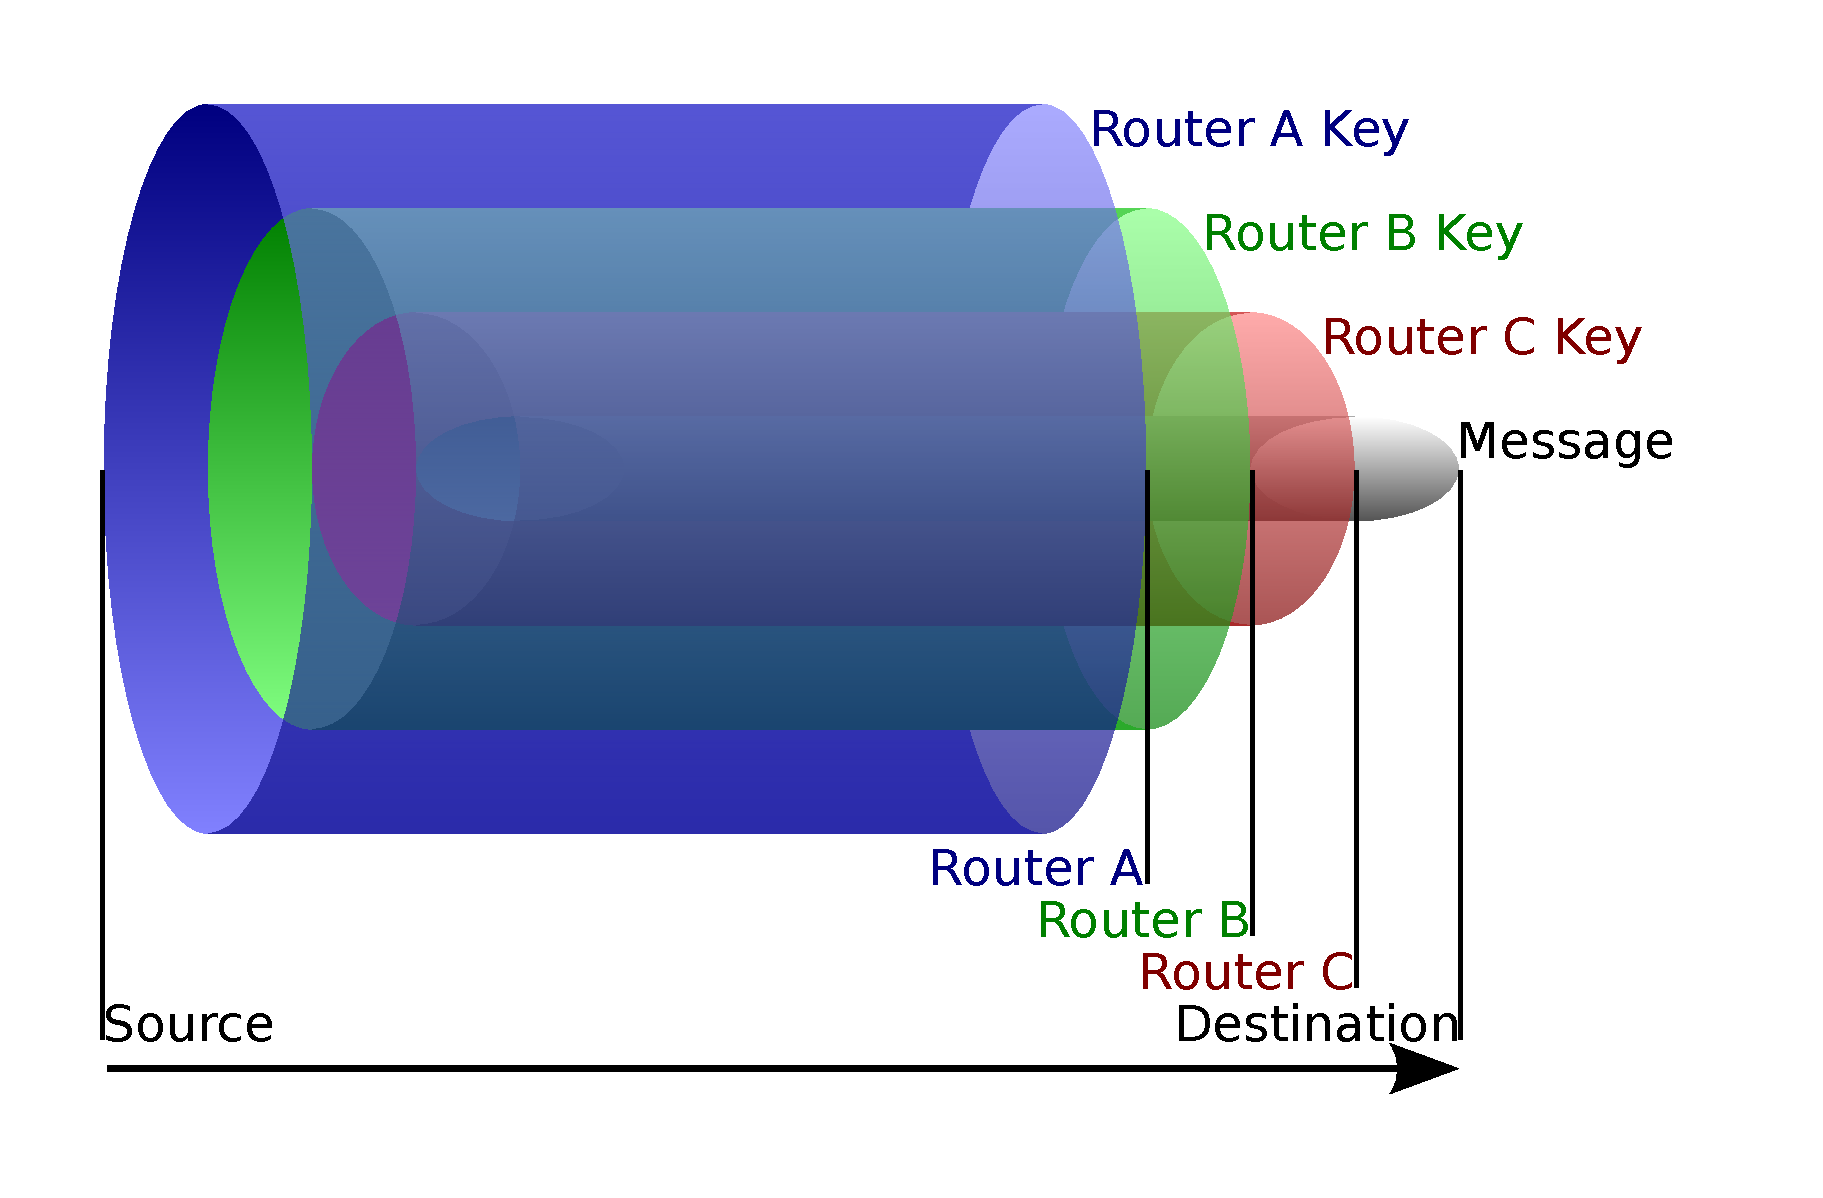
\includegraphics[width=\textwidth]{Onion_diagram.pdf}
\caption{Warstwy szyfrowania (autor:  HANtwister, Wikipedia\cite{wikionion})}
\end{figure}

\subsection{TOR}
Implementacją trasowania cebulowego jest TOR(Tor Onion Router), czyli stworzone w 
latach 2002-2004 oprogramowanie oraz sieć routerów, dostęne nie tylko dla agencji 
rządowych, ale także dla osób prywatnych, chcących zachować prywatność lub anonimowość.
Tor może być używany jako proxy między użytkownikiem a całą resztą ``zwykłego'' 
internetu, ale oferuje także możliwość wystawienia servera(TOR hidden service), 
który będzie widoczny tylko dla użytkowników sieci TOR. Dużą zaletą tego 
rozwiązania jest szyfrowanie end-to-end, dzięki czemu nawet po zdjęciu warstwy 
szyfrowania odpowiadającej ostatniemu routerowi, mamy gwarancję że nie będzie on w 
stanie odczytać wysyłanej wiadomości.
\par
Zanim przyjrzymy się tej technologii z bliska, warto rozwiać pewne wątpliwości.
Większość ludzi którzy słyszeli o TORze, zapewne zetknęła się z opinią, że jest to sieć 
służąca wyłącznie do nielegalnych celów, takich jak udostępnianie pornografii dziecięcej
bądź handel narkotykami. Gdyby tak było, żadnemu przestępcy nie opłacałoby się używać TORa,
dlatego że jeśli służby zauważyłyby że ktoś go używa, to najprawdopodobniej jest on przestępcą.
Można w takim razie się zastanawiać, dlatego używanie TORa jest legalne? Czy zdelegalizowanie go
nie ułatwiłoby pracy służbom? Roger Dingledine, współtwórca TORa wypowiedział się o tym w 
następujący sposób:

\begin{quote}
\textit{The United States government can’t simply run an anonymity system for everybody and then 
use it themselves only. Because then every time a connection came from it people would say, 
``Oh, it’s another CIA agent.'' If those are the only people using the network.}
\end{quote}


Należy pamiętać że służbom także zależy na anonimowości i prywatności. Gdyby istniał 
odpowiednik TORa używany jedynie przez agencje rządowe, służby z innych krajów prędzej 
czy później dowiedziałyby się o adresach IP przekaźników tej sieci, przez co cała
technologia stałaby się kulą u nogi. Wniosek z tego jest taki, że aby istniała 
anonimowość, musi też istnieć różnorodność. W interesie każdej osoby używającej TORa jest to,
aby korzystali też z niego inni, a wzajemne zwalczanie się jest nikomu nieopłacalne.

\section{TOR od strony technicznej}
\subsection{Struktura sieci}
Sieć TOR charakteryzuje się tym że jest hybrydą między systemem rozproszonym a 
scentralizowanym. Routery, nazywane często przekaźnikami(ang. Relay), są tworzone
przez społeczność. Każdy może stworzyć własny router, przez który będą się łączyć 
inni użytkownicy. Jak w takim razie dowiedzieć się o ich istnieniu? Tutaj pojawia 
się scentralizowana część sieci. Na świecie istnieje 10 uprzednio wybranych(rys. 2), 
zaufanych węzłów(directory authorities). Co godzinę, każdy z nich uczestniczy w głosowaniu, 
poprzez które ustalają jak ma wyglądać cała sieć. Skutkiem głosowania jest tzw. 
consensus, czyli dokument tekstowy opisujący wynik głosowania. Mogą oni faworyzować
niektóre przekaźniki, opierając się np. na przepustowości ich łącza lub czasie
działania. Przykładowo, jako pierwszy węzeł na trasie można wybierać jedynie te węzły
którym została przyznana specjalna flaga. Aby ją zdobyć, przekaźnik musi działać
przez około 8 dni, oraz posiadać stabilne łącze. Jest to spowodowane tym, że węzły 
tego typu znają prawdziwy adres IP użytkownika, a więc są one duża bardziej krytyczną
częścią infrastruktury niż np. węzły  na środku trasy.

\begin{figure}
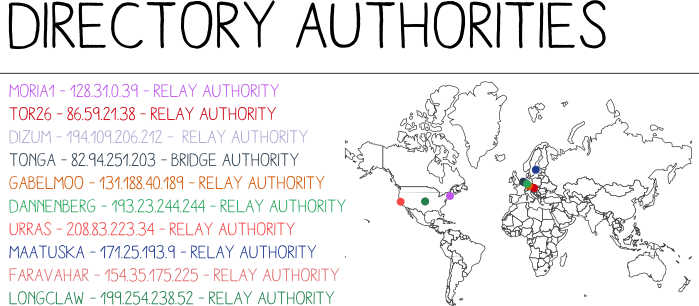
\includegraphics[width=\textwidth]{authorities.png}
\caption{directory authorities (autor:  Jordan Wright\cite{consensus})}
\end{figure}

\subsection{Trasa komunikacji}
Nawiązując połączenie z siecią TOR, wybieramy losowo pierwszy węzeł(guard node),
a następnie używamy protokołu Diffiego-Hellmana(lub któregoś z jego wariantów) aby 
ustalić wspólny sekret. Od tego momentu połączenie między użytkownikiem a pierwszym
routerem jest szyfrowane. Używając pierszego węzła jako proxy, powtarzamy ten proces, 
i nawiązujemy połączenie z drugim(middle node) oraz trzecim(exit node) węzłem.
Warto wspomnieć, że TOR nigdy nie ukrywał, i nigdy nie miał zamiaru ukrywać faktu
iż dana osoba z niego korzysta, dlatego warto mieć na uwadze, że nasz dostawca 
internetu ma wiedzę o tym że lączymy się z TORem. Nie oznacza to jednak utraty
ani anonimowości, ani prywatności, dlatego że zarówno nasz dostawca internetu, jak 
i pierwszy router na trasie nie wiedzą z kim i w jakim celu się komunikujemy.
Router środkowy widzi jedynie że dwa przekaźniki wewnątrz sieci komunikują się
między sobą, zatem nie zna ani nadawcy ani odbiorcy. Trzeci router jest nieco 
groźniejszy, dlatego że zna on odbiorcę wiadomości(nie zna nadawcy), a także
jest odpowiedzialny za zdjęcie ostatniej warstwy szyfrowania, co narusza prywatność,
o ile nie użyjemy innych środków zapewniających szyfrowanie end-to-end.
Niestety, nie jest to takie proste. Potrzebne jest założenie że każdy
z tych trzech węzłów jest niezależny(tzn. każdy jest kontrolowany przez inną 
osobę bądź organizację, które nie są ze sobą powiązane). Według twórców 
TORa\cite{secondgeneration}, jest to jedno z największych zagrożeń dla anonimowości.
O ile nie istnieje złoty środek który sprawi że problem zniknie, istnieją metody 
sprawiające że ataki opierające się na kontrolowaniu więcej niż jednego węzła na trasie
stają się trudne. Przykładem może być ``przypięcie'' pierwszego routera na trasie do 
klienta na długi okres czasu(rzedu dwóch miesięcy). Dzięki temu, co prawda część 
użytkowników może wybrać węzły należące do adwersarza, ale za to wszyscy pozostali,
przez cały ten czas bedą bezpieczni. Argument stojący za tym rozwiązaniem jest taki,
że  wykonanie jednokrotnego ataku deanonimizującego klienta juz serwer, jest tak samo 
złe jak możliwość wykonywanie takich ataków przez dłuższy okres czasu. Korzyść nie jest
oczywista, ale powstały pracę naukowe\cite{entryguard}, w których autorzy wykazali 
że system ten zapewnia większe bezpieczeństwo niż ten klasyczny.

\subsection{Ukryte usługi}
Jak już zostało powiedziane, użytkownicy mogą używać TORa jako proxy, dzięki czemu
odbiorca nie jest w stanie dowiedzieć się kim jest nadawca. A co jeśli ktoś chce
świadczyć usługi jako serwer, pozostając anonimowym? TOR przewiduje także taką możliwość,
używając usług ukrytych(and TOR hidden services), widocznych jedynie dla klientów 
używających TORa. Rozważmy scenariusz gdzie Bob staje się serwerem, a Alice, jako 
klient, chce nawiązać z nim połączenie. Aby tego dokonać\cite{deanonymisation}, 
Bob losowo wybiera 3 przekaźniki z całej sieci TOR, czyli tzw. punkty wprowadzenia(ang. 
introduction points), a następnie nawiązuje z nimi połączenie, tak jak zostało to 
opisane wcześniej. Węzły te będa później potrzebne  do nawiązania połączenia z klientem.
Najpierw, Bob generuje parę kluczy RSA, z użyciem klucza długości 1024 bitów. Nie jest
to jeszcze kryptografia którą można z łatwością złamać, ale jest to zdecydowanie za mało,
ale twórcy planują\cite{tortalk} zastąpienie 1024-bitowego RSA przez silniejsze 
algorytmy, oparte na krzywych eliptycznych(ED25519).
Następnie, Bob oblicza $SHA1$ klucza publicznego, z czego pierwsze 10 bajtów stają się 
identyfikatorem ukrytej usługi($HS_{id}$). 
Od teraz adresem usługi Boba jest $base32(HS_{id}).onion$. Aby usługa Boba była dostępna 
dla reszty sieci, musi on udostępnić im deskryptor swojej usługi, czyli plik tekstowy,
zawierający informację potrzebne do nawiązania połączenia, m.in. klucz publiczny. 
W sieci TOR, niektóre węzły pełnią rolę baz deskryptorów usług ukrytych(ang. hidden service 
directory), czyli po prostu przechowują te deskryptory, a także 
dostarczają je klientom, gdy ci o to poproszą. Bob, jako serwer, będzie musiał wybrać 
odpowiadający adresowi jego usługi węzeł, któremu będzie mógł udostępnić swój deskryptor. 
Aby to zrobić, Bob oblicza identyfikator deskryptora($desc_{id}$) w następujący sposób
($\|$ oznacza konkatenację):
\begin{center}
$desc_{id} = H(address \| H(timestamp \| desc_{cookie} \| replica))$
\end{center}
Gdzie $H$ to funkcja haszująca(aktualnie jest to SHA1, ale planuje się\cite{tortalk}
zastąpienie jej przez SHA3),
$address$ jest adresem Boba, opisanym wcześniej, $timestamp$ to ilość dób od 
początku epoki UNIXa. $desc_{cookie}$ ma znaczenie tylko gdy chcemy ograniczyć dostęp 
do usługi tylko do ludzi znających ciasteczko, zazwyczaj to pole jest puste.
$replica$ to liczba(zazwyczaj 1 lub 0), służąca do wyboru zbioru węzłów przechowujących
deskryptor serwera. Aby wybrać odpowiadający węzeł, Bob sortuje fingerprinty wszystkich
węzłów-kandydatów(fingerprintem węzła jest fingerprint jego klucza publicznego) 
na przechowywanie deskryptora usługi Boba, a następnie wybiera 
3 następne, które są większe(leksykograficznie) od identyfikatora deskryptora 
Boba(jeśli takich nie ma to wybieramy te z początku listy),
tzn. z ciągu:
\begin{center}
$HSdir_{n-2}, HSdir_{n-1}, desc_{id}, HSdir_{n}, HSdir_{n+1}, HSdir_{n+2}$
\end{center}
Bob wybierze $HSdir_{n}, HSdir_{n+1}, HSdir_{n+2}$. Od teraz Alice, znając adres
Boba może nawiązać połączenie, robi to w następujący sposób:

\begin{enumerate}
\item Alice dowiaduje się o adresie usługi Boba w jakikolwiek sposób(poprzez wyszukiwarkę,
bezpośrednio od Boba).
\item Alice wybiera losowo, z całej sieci TOR tzw. punkt spotkania(ang. rendezvous point), 
nawiązuje z nim połączenie, oraz generuje losowe ciasteczko.
\item Alice wyznacza węzeł zawierający informację o usłudze Boba na podstawie jego
adresu, a następnie pobiera z niego informacje dotyczące punktów wprowadzenia
\item Alice buduje nowe połączenie z jednym z punktów wprowadzenia, wysyła zaszyfrowane
kluczem publicznym Boba adres IP, fingerprint punktu spotkania, oraz sekretne ciasteczko
\item Punkt wprowadzenia przekazuje wiadomość do Boba, który po odszyfrowaniu wiadomości,
nawiązuje połączenie z punktem spotkania i przekazuje mu ciasteczko.
\end{enumerate}

Od teraz Alice komunikuje się z Bobem poprzez punkt spotkania, używając szyfrowania end-to-end. 
Obie strony łączą się z nim poprzez TOR, a więc anonimowość jest zapewniona zarówno
dla serwera jak i klienta. Ciekawą cechą związaną z usługami ukrytymi jest to że nie 
trzeba konfigurować usługi NAT, dlatego że to serwer jako pierwszy nawiązuje połączenie
z punktem spotkania.

\section{Zagrożenia dla TORa}
Niestety, okazuje się że system opisany w powyższym rozdziale ma wiele pułapek które
mogą naruszyć anonimowość lub prywatność użytkowników. Nie oznacza to jednak że cała
idea jest zła, lub że używanie TORa nie ma sensu, dlatego że zazwyczaj takie ataki
wymagają dość dużych środków i zaangażowania, a nawet wtedy nie ma pewności że uda się
coś na tym ugrać. Z drugiej strony, nie da się ukryć że istnieją organizację które takie
środki posiadają, dlatego warto przyjrzeć się problemom z którymi muszą zmagać się
twórcy TORa.
\subsection{Deanonimizacja klienta}
Opisywana metoda polega na analizie odstępów czasowych między poszczególnymi działaniami
klienta, oraz nosi nazwę HSDir deanonymization attack\cite{tortalk}.
Rozważmy sytuacje w której Alice jest klientem chcącym połączyć się z pewną usługą 
ukrytą, a Eve jest pasywnym adwersarzem, kontrolującym guard node powiązany z Alice,
oraz oraz węzeł przechowywyjący deskryptor usługi ukrytej z którą chce się połączyć
Alice. Eve może przeprowadzić atak czasowy, obesrwując proces łączenia się Alice z
usługą ukrytą, wyglądający następująco(podane odstępy czasowe nie muszą zawsze być takie,
jest to jedynie przykład, ale wydają się one dość prawdopodobne):
\begin{enumerate}
\item $(15:34:03)$ Alice tworzy połączenie z węzłem przechowującym interesujący ją
deskryptor usługi ukrytej
\item $(15:34:05)$ Eve odnotowywuje żądanie dla pewnego deskryptora umieszczonego na
jej serwerze
\item $(15:34:06)$ Alice zamyka poprzednio otwarte połączenie
\item $(15:34:06)$ Alice otwiera połączenie do punktu spotkania
\item $(15:34:06)$ Alice otwiera połączenie do punktu wprowadzenia
\item $(15:34:08)$ Alice zamyka połączenie z punktem spotkania
\item $(X:Y:Z)$ Alice komunikuje się z punktem spotkania przez pewien okres czasu(tzn. 
nie zabija połączenia natychmiastowo)
\end{enumerate}

Warto przypomnieć, że Eve nie wie o tym czy Alice łączy się z punktem spotkania, czy 
z jakimkolwiek innym punktem, odnotowuje ona jedynie fakt zaistnienia pewnego połączenia 
zainicjowanego przez Alice. Obserwując tego typu ruch, Eve może skojarzyć adres IP
Alice z serwisem którego deskryptor został własnie pobrany, czyli stwierdzić z dość
dużym prawdopodobieństwem że Alice łączy się z pewnym serwerem z sieci TOR.

\subsection{Deanonimizacja serwera}
Załóżmy że Bob prowadzi usługę ukrytą w sieci TOR, a Eve kontroluje guard node przez
który Bob łączy się z resztą sieci, oraz pewien inny przekaźnik, który może posłużyć
jako punkt spotkania. Eve przypuszcza że Bob prowadzi sklep z narkotykami, ale 
chciałaby to w jakiś sposób potwierdzić. Atak wygląda następująco:

\begin{enumerate}
\item Eve wysyła do punktu wprowadzenia sklepu narkotykowego informacje o chęci nawiązania
połączenia, oraz kontrolowanego przez nią adres punktu spotkania.
\item Bob nawiązuje połączenie z podanym punktem spotkania, powiadamiając go o gotowości na 
nawiązanie komunikacji
\item Po otrzymaniu powiadomienia przez punkt spotkania, Eve odsyła do jego nadawcy $N$
pakietów, mających służyć jako padding, który serwer odrzuci.
\item Eve wysyła z punktu spotkania informację o zakończeniu połączenia.
\end{enumerate}

Guard node należący do Eve cały czas monitoruje ruch, więc jest w stanie stwierdzić, że
z dużym prawdopodobieństwiem należy do Boba, o ile tylko uda się skorelować 
próbe nawiązania połączenia ze sklepem narkotykowym Boba z następującym ciągiem 
wiadomości(wysyłanie trzech pakietów wynika ze specyfikacji protokołu):

\begin{enumerate}
\item Wiadomość o gotowości do komunikacji(3 pakiety w stronę punktu spotkania)
\item Wiadomość o zakończeniu połączenia(3 pakiety w stronę serwera)
\item $N$ pakietów paddingu w stronę serwera
\end{enumerate}

Może się wydawać że taki atak może się nie udać przez to że oprócz pakietów wysyłanych
przez atakującego, przez przekaźniki przesyłają informację także inni użytkownicy,
ale jak pokazują badania\cite{deanonymisation}, ta technika może być praktycznie 
bezbłędna.

\subsection{Naruszanie prywatności}
Jak już zostało wspomniane, przekaźnikiem może być każdy, w szczególności każdy(spełniając
pewnie wymagania) może być przekaźnikiem przechowującym deskryptory usług ukrytych. Każdy z
deskryptorów przechowuje klucz publiczny, za pomocą którego można wyliczyć adres serwisu, 
metodą opisaną w poprzednim rozdziale. Osoba kontrolująca taki przekaźnik, może zbierać adresy
usług ukrytych, a także minitorować ruch, co nie powinno mieć miejsca w sieci takiej jak TOR.
Twórcy TORa twierdzą\cite{tortalk}, że jest to bardzo szkodliwe, oraz że istnieją setki firm, których model
biznesowy opiera się o takie działanie. Mogą one wtedy wysyłać crawlery, zbierające dane o całej sieci.






\section{Czy ludzie potrafią korzystać z TORa?}
W poprzednim rozdziale przyglądaliśmy się technicznym atakom na uczestników sieci TOR. 
Okazuje się jednak, że wcale nie są one potrzebne, dlatego że z powodu niewiedzy bądź głupoty,
ludzie sami potrafią ujawnić swoją tożsamość, i nie trzeba używać do tego żadnych
zaawansowanych technologii.
\par 
Jak podaje portal forbes.com\cite{harvardstudent}, pod koniec
roku 2013 pewien student Harvardu postanowił zawiadomić policję o tym że na uczelni 
jest bomba. Oczywiście, żadnej bomby nie było, a cały ten donos to próba uniknięcia
egzaminu, dlatego student postanowił że zadba o to aby policja nie dowiedziała się 
o jego tożsamości. Z tego powodu, postanowił on wysłać maila z donosem, używając TORa.
Niestety, nie wiedział o tym, że używając sieci bezprzewodowej udostępnianej przez jego
uczelnie, która do autentykacji wymaga imienia i nazwiska, w logach serwera znajdzie 
się informacja o tym że że komunikował się poprzez sieć TOR. Można domyślać się, 
że w czasie wysyłania maila, był on jedyną osobą z tej sieci używającą TORa, 
dlatego że policja nie miała większego problemu z namierzeniem sprawcy. 
\par
Nie mogło także zabraknąc historii twórcy portalu Silkroad, Rossa Ulbrichta. Zaufana Trzecia
Strona\cite{z3sulbricht} opisuje dokładnie wszystkie jego wpadki. 
Zaczęło się 27. stycznia, 2011 r., od 
poinformowania o istnieniu nowego serwisu handlującego narkotykami na forum 
internetowym shroomery.org, przez użytkownika o pseudonimie altoid. Podobna sytuacja
zdarzyła się dwa dni później, gdy użytkownik o tym samym pseudonimie umieścił podobną
informację na forum bitcointalk.org. 8 miesięcy później, ten sam użytkownik umieścił 
ogłoszenie w którym oferuje pracę w startupie, w której wymagał specjalistycznej wiedzy
o Bitcoinie. Tym razem podał on swój adres email - rossulbrich@gmail.com.
Ustalono że w kodzie serwera Silkroad istnieje zabezpieczenie, ograniczające dostęp
do panelu administacyjnego do jednego numeru IP. FBI znało ten adres, oraz ustaliło
że należy on do serwera jednego z dostawców VPN, który wyjawił ostatnio adres IP 
z którego łączona się z tym serwerem. Okazało się że jest to adres kawiarenki 
internetowej, a jak potem udało się ustalić, z tego samego adresu IP logowano się
na skrzynkę mailową Rossa Ulbrichta. Kolejną wpadką twórcy Silkroad'a było
zamawianie fałszywych dowodów na swój adres zamieszkania. Przesyłka została 
przechwycona na granicy z Kanadą, wszystkie dokumenty zawierały zdjęcie przedstawiające
Rossa Ulbrichta, ale z innymi danymi osobowymi. Nie są to wszystkie jego wpadki, ale 
myślę że jest to wystarczająco dużo, a szczególnie dla FBI, by mieć pewność że jest
on co najmniej zamieszany w zarządzenie Silkroadem. Historia Rossa Ulbrichta kończy 
się w październiku 2013r., kiedy został zatrzymany w bibliotece publicznej w 
San Francisco, gdzie agenci FBI przechwycili jego (włączony) komputer, na którym 
był on zalogowany do panelu administacyjnego Silkroad.
\par
Jak widać, w wyżej opisanych przypadkach ani razu nie wykorzystano błędów w technologii,
a nawet nie potrzeba było stosować wyrafinowanej socjotechniki. 
Przestępcy zostawiali po sobie tyle poszlak, że wystarczyło jedynie trochę poszukać, by ich 
odnaleźć. Warto jest o tym pamiętać, jeśli ktoś próbuje argumentować nieskuteczność TORa 
tym, że dużo ludzi wpadło, mimo że z niego korzystali. Technologia to nie talizman, który
ma zapewnić nam ochronę, ale narzędzie z którego należy umiejętnie korzystać.


\begin{thebibliography}{99}

\bibitem{onioncreation} Reed M. G., Sylverson P. F., Goldschlag D. M. (1998), 
\textit{Anonymous connections and onion routing},
IEEE Journal on Selected Areas in Communications, 16(4):482-494

\bibitem{wikionion} HANtwister, 
\textit{Onion routing},
\url{https://en.wikipedia.org/wiki/Onion_routing},
[odwiedzone 17.12.2017]

\bibitem{consensus} Jordan Wright
\textit{How Tor Works Part Three - The Consensus},
\url{https://jordan-wright.com/blog/2015/05/14/how-tor-works-part-three-the-consensus/},
[odwiedzone 17.12.2017]

\bibitem{secondgeneration} Roger Dingledine, Nick Mathewson, Paul Syverson
\textit{Tor: The Second-Generation Onion Router}

\bibitem{entryguard} Tariq Elahi
, Kevin Bauer
, Mashael AlSabah
, Roger Dingledine
, Ian Goldberg
\textit{Changing of the Guards: A Framework for Understanding and Improving Entry 
Guard Selection in Tor}

\bibitem{deanonymisation} Alex Biryukov,
Aaron Johnson,
Jean-Sébastien Coron, 
Thorsten Holz,
Ralf-Philipp Weinmann, 
\textit{Deanonymisation techniques for Tor and Bitcoin (12/06/2015) }

\bibitem{tortalk} asn, 
Nima Fatemi, 
David Goulet,
\textit{Understanding Tor Onion Services and Their Use Cases - HOPE XI 2016}

\bibitem{harvardstudent} Runa A. Sandvik (18/12/2013),
\textit{Harvard Student Receives F For Tor Failure While Sending Anonymous Bomb Threat}
\url{https://www.forbes.com/sites/runasandvik/2013/12/18/harvard-student-receives-f-for-tor-failure-while-sending-anonymous-bomb-threat}
[odwiedzone 19.12.17]

\bibitem{z3sulbricht} Adam Haertle (03/11/2013),
\textit{Seria wielu drobnych wpadek, czyli jak FBI namierzyło założyciela Silk Road}
\url{https://zaufanatrzeciastrona.pl/post/seria-wielu-drobnych-wpadek-czyli-jak-fbi-namierzylo-zalozyciela-silk-road/}
[odwiedzone 19.12.17]


\end{thebibliography}

\end{document}
